%%%%             %%%%
%%%% METODOLOGÍA %%%%
%%%%             %%%%

% TODO explicar cómo facilita Scrum la adaptación para la construcción del prototipo web

\chapter{Metodología}
\label{chap:metodologia}

\lettrine{E}{ste} capítulo trata sobre metodologías aplicadas a proyectos de software y en particular la metodología seleccionada para el este trabajo, Scrum.

Las metodologías que se refieren al Ciclo de Vida del Desarrollo de Software, SDLC en inglés, son procesos y prácticas utilizadas por los equipos de desarrollo de software para tratar con éxito el SDLC.

Históricamente la metodología más conocida es la metodología de desarrollo en Cascada, que tiene su origen en un artículo científico de Winston W. Royce en los años 70. Esta metodología se completa en cinco etapas:

\begin{enumerate}
    \item Análisis de requisitos
    \item Diseño
    \item Implementación
    \item Verificación
    \item Mantenimiento
\end{enumerate}

Un proyecto se realiza en un único ciclo,  las etapas se ejecutan en orden y sin solapamientos. Este es un modelo que resulta rígido e impone muchas limitaciones: las pruebas de integración no se pueden llevar a cabo hasta completar todo el desarrollo, los usuarios no puede probar la aplicación hasta el final del proyecto, que se puede demorar meses o incluso años. En este modelo no hay oportunidad para que los clientes u otras partes interesadas puedan ofrecer sus opiniones.

Para tratar de ofrecer una alternativa a las limitaciones impuestas por el desarrollo en cascada, fueron propuestas otras metodologías, como la metodología en espiral o la metodología en V. Pero no fue hasta mediados de los años 90, que no aparecen las primeras tecnologías ágiles. Especialmente, en el año 2001, se publicó el Manifiesto por el desarrollo ágil que valora los siguientes cuatro puntos:

\begin{itemize}
    \item Individuos e interacciones sobre procesos y herramientas.
    \item Software funcionando sobre documentación extensiva.
    \item Colaboración con el cliente sobre negociación contractual.
    \item Respuesta ante el cambio sobre seguir un plan.
\end{itemize}

En este proyecto se utiliza Scrum que pertenece al conjunto de metodologías ágiles.

\section{Scrum}

\emph{The Scrum Guide} es la guía oficial donde se presenta el \emph{framework} Scrum. Scrum es un marco de trabajo para ayudar en la creación de valor mediante soluciones adaptativas a problemas complejos. Scrum propone una filosofía general, varios roles para las tareas, unos eventos que se repiten de forma cíclica y unos artefactos como producto del trabajo.

Scrum no está limitado a proyectos de software. Siempre y cuando se respeten sus características, se posiciona como un modelo más general, que se puede aplicar a cualquier proyecto donde sea capaz de aportar valor.

\subsection{Roles}

La unidad de trabajo está formada por el Equipo Scrum. Se consideran tres roles dentro del Equipo:

\begin{itemize}
    \item Los \textbf{Desarrolladores} son todas las personas que contribuyen a crear los incrementos durante cada ciclo. Las cualidades de las personas consideradas desarrolladoras pueden ser variadas. Los desarrolladores son responsables del mantenimiento del Sprint Backlog.
    \item El \textbf{Product Owner} es la persona responsable de maximizar el valor resultante del trabajo del Equipo Scrum. El \emph{framework} no indica como debe conseguirse este objetivo. El Product Owner también es responsable del Product Backlog.
    \item El \textbf{Scrum Master} es responsable de asegurar que se siguen los principios del marco de trabajo y entre sus obligaciones está la de actuar apoyando a los demás miembros del equipo para la mejora de las prácticas relacionadas con Scrum. De forma general es responsable de la efectividad del Equipo.
\end{itemize}

\subsection{Eventos}

El ciclo de vida de Scrum está contenido en el Sprint. Durante un Sprint se lleva a cabo el trabajo generador de valor para el proyecto. La duración de un Sprint es flexible pero debería estar entre una y cuatro semanas. Debe ser lo suficientemente largo como para dar tiempo a la realización de trabajo significativo, pero no tan largo que se pierda de vista el objetivo del propio Sprint, o que el objetivo planificado cambie y ya no sea válido. Dentro del Sprint se suceden los otros cuatro tipos de eventos.

\begin{figure}[hp!]
    \centering
    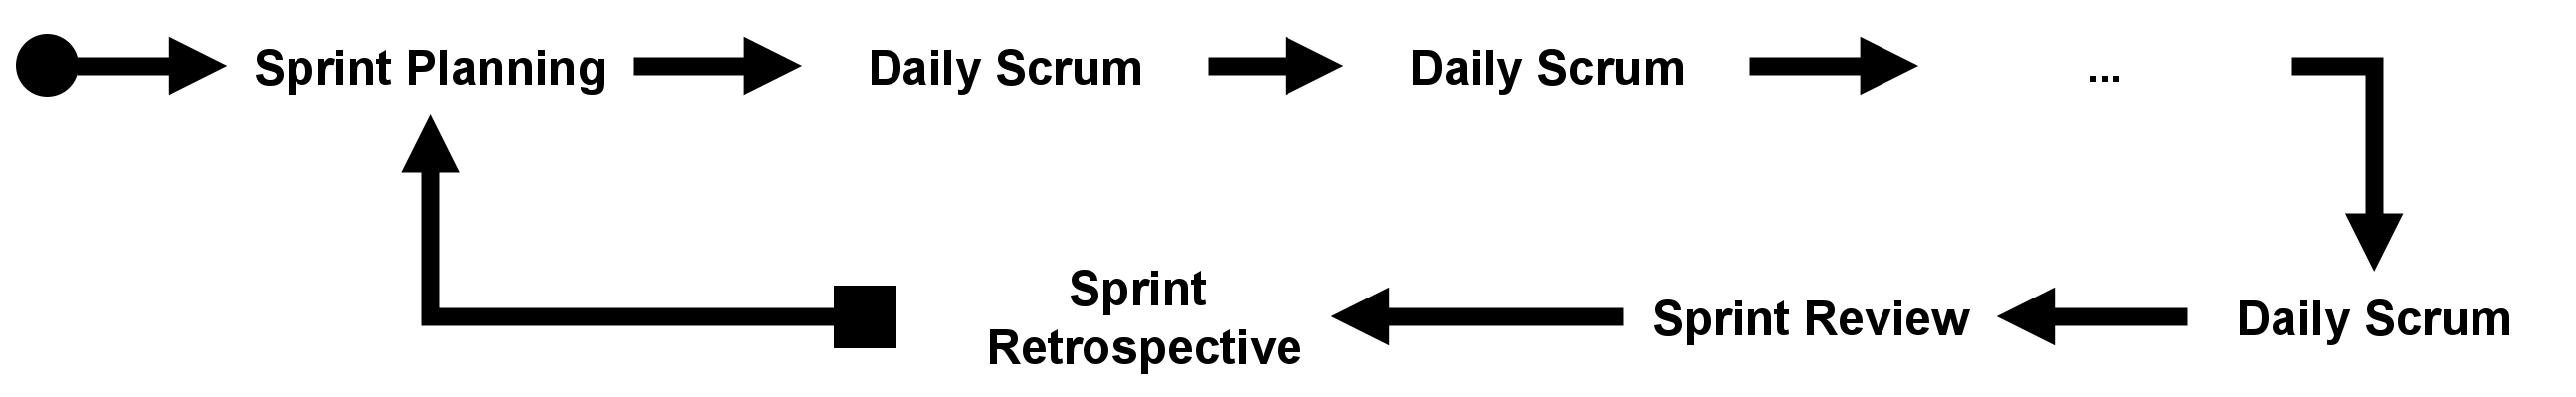
\includegraphics[width=1.0\textwidth]{imaxes/d-metodologia/ciclo-scrum.png}
    \caption{Ciclo de vida de Scrum}
    \label{fig:ciclo-vida-scrum}
\end{figure}

\begin{itemize}
    \item El \textbf{Sprint Planning} da comienzo a un nuevo Sprint. En este evento se acuerda el trabajo que se va a realizar durante el Sprint. El Equipo completo trabaja para establecer las tareas particulares que serán abordadas en el periodo. En el Sprint Planning pueden participar otras personas involucradas con el proyecto, pero que no pertenezcan al Equipo. Su ayuda puede ser necesaria para aclarar aspectos de las tareas o los objetivos.
    En este evento es importante dar respuesta a cómo se puede añadir más valor al producto. El Objetivo del Sprint debe quedar claramente definido y para ello todo el equipo colabora. También hay que establecer qué cosas se pueden llevar a cabo durante el Sprint. Se seleccionan por tanto todas aquellas tareas que deberán ser abordadas. Por último se requiere decidir cómo se llevarán a cabo las tareas. Puede ser necesario conseguir un mayor refinamiento para que los Desarrolladores puedan tomar las decisiones correspondientes.

    \item El \textbf{Daily Scrum} es un evento de 15 minutos para revisar el avance hacia el objetivo del Sprint. Como en otros aspectos de Scrum, el \emph{framework} no explicita la técnica o estructura de la reunión, pero insiste en que es el momento de comunicar dificultades, logros y planificar el trabajo para la jornada siguiente. A esta reunión solo acuden los Desarrolladores.
    
    \item El \textbf{Sprint Review} tiene por objetivo analizar y enseñar las mejoras alcanzadas durante el Sprint. A esta reunión acudirá no solo el Equipo sino también todas las personas involucradas de forma amplia. Esta sesión no solo es de exposición, también sirve para decidir futuras adaptaciones. De hecho, Scrum propone este momento para seleccionar cuáles son las \emph{features} que se completarán a continuación.
    
    \item El \textbf{Sprint Retrospective} se propone como una reunión para mejorar la calidad y la efectividad. Esta es una oportunidad para revisar todos los componentes del proceso de trabajo y encontrar problemas en procesos, herramientas, comunicaciones, etc. La reunión debe responder a qué cosas fueron bien, cuáles fueron mal y como se gestionaron. Se deben proponer acciones de mejora para los problemas. Si es oportuno, estas acciones podrían ser incluidas en el Sprint Backlog.
\end{itemize}

\subsection{Scrum Artifacts}

Los Artefactos son la representación del trabajo o del valor. Cada uno de los artefactos está relacionado con un compromiso en el proyecto.

\begin{itemize}
    \item El \textbf{Producto Backlog} es la lista priorizada de todo aquello que debe realizarse para mejorar el producto. Es la fuente de trabajo utilizada por el Equipo. Todos los elementos que quepan dentro de un Sprint son susceptibles de ser incorporados al Sprint Backlog.
    \item El \textbf{Sprint Backlog} contiene el Objetivo del Sprint, un subconjunto del trabajo existente en el Project Backlog y que será el trabajo acometido durante el Sprint. Por último, contendrá un plan de trabajo para conseguir aportar el valor al proyecto.
    \item Los \textbf{Incrementos} son las unidades que hacen avanzar hacia en Objetivo del Proyecto. Puede ser cualquier cosa siempre y cuando se comporte de manera aditiva a todos los demás Incrementos y sea utilizable. Los incrementos deben funcionar de forma conjunta, así que serán revisados con el objetivo de comprobar su calidad.
\end{itemize}

De forma general Scrum es un proceso en cuatro etapas:

\begin{enumerate}
    \item El Product Owner toma un problema complejo y lo transforma en unidades individuales de trabajo.
    \item El Equipo Scrum realiza una selección del trabajo y lo transforma en un Incremento de valor durante un Sprint.
    \item El Equipo y otras partes interesadas revisar los resultados y ajustan todo lo necesario para el siguiente Sprint.
    \item Se vuelve a empezar.
\end{enumerate}

\section{Uso de Scrum en el proyecto}
\label{sec:uso-scrum-en-el-proyecto}

Para la aplicación del Scrum a proyecto han sido necesarias algunas adaptaciones por la propia naturaleza del TFG. El rol de Product Owner lo ha realizado el director del proyecto. El Equipo de Desarrollo está formado únicamente por el alumno, que también ha hecho las funciones de Scrum Master.

Las reuniones se han reducido, al no existir otras personas con las cuales coordinarse. Se han mantenido las reuniones con el director del proyecto para la revisión del Sprint y el Sprint Planning. Las reuniones se han llevado a cabo de forma telemática.

El comienzo del proyecto se ha recurrido al concepto de Spike para la adquisición de conocimiento. Un Spike es una historia de usuario especialmente indicada para dar tiempo al Equipo a explorar una tecnología desconocida, comprender una implementación con la que no se está familiarizado, elaboración de prototipos o cualquier otra necesaria para poder completar avanzar el proyecto.

\section{Herramientas de apoyo a la metodología}

Para la planificación del proyecto se recurrió a Microsoft Project 2013. Si bien esta herramienta permite obtener una visión completa del trabajo y realizar su seguimiento, no resulta tan práctica a la hora de desgranar las tareas a un nivel más fino.

Para organizar las historias de usuario y poder dividir el trabajo en tareas se empleó el servicio web Github \footnote{\url{https://github.com/}}. Asociado a cada repositorio de código se puede crear un tablero para organizar las tareas, el espacio se divide en columnas, que representan historias de usuario. También se creó una columna para representar el trabajo en curso y tantas columnas como Sprints para ir colocando las tareas realizadas. Una parte del tablero se puede ver en la Imagen \ref{fig:tablero-github}.

\begin{figure}[hp!]
	\centering
	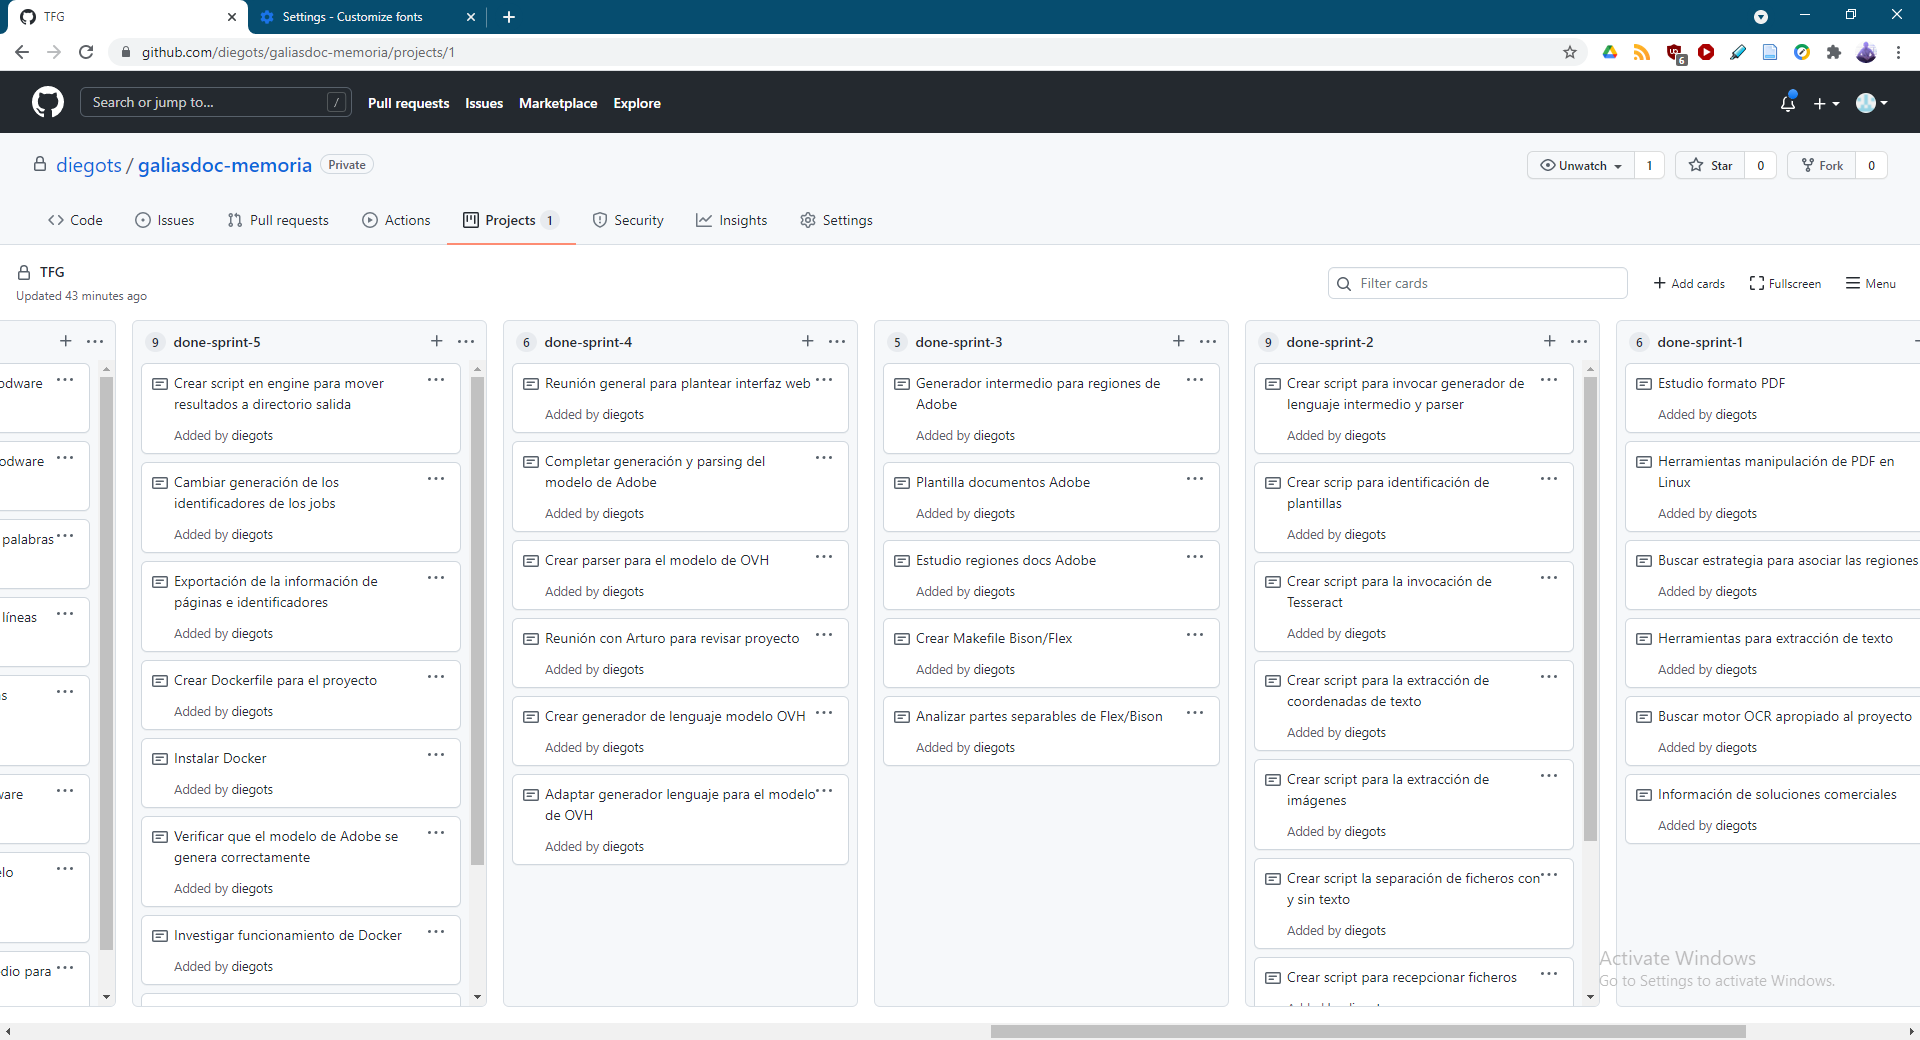
\includegraphics[angle=90,width=0.70\textwidth]{imaxes/f-planificacion/tablero-planificacion}
	\caption{Tablero en Github con las tareas del proyecto}
	\label{fig:tablero-github}
\end{figure}